\section{Additional Results}\label{app:traces}
\subsection*{Cycle results for all initial SOC values}
\begin{table}[H]
\centering
\caption{Loss energies in kWh (conduction, switching, battery) and cycle efficiency of both drives for initial SOC of \SIlist{20;50;90}{\percent}.}
\label{tab:resfull}
\footnotesize
\setlength\tabcolsep{3pt}
\begin{tabular}{@{}lrrrrrrrrrr@{}}
\toprule
 & & \multicolumn{3}{c}{2L [kWh]} & \multicolumn{3}{c}{BI-MMC [kWh]} & \multicolumn{2}{c}{$\etacyc$ [\%]} & \\
Application & SOC [\%] & $E_\mathrm{c}$ & $E_\mathrm{s}$ & $E_\mathrm{b}$ & $E_\mathrm{c}$ & $E_\mathrm{s}$ & $E_\mathrm{b}$ & 2L & BI & $\Delta\etacyc$ [pp] \\
\midrule
Passenger car & 20 & 0.024 & 0.018 & 0.019 & 0.014 & 0.004 & 0.081 & 98.75 & 97.98 & -0.77 \\
 & 50 & 0.021 & 0.018 & 0.015 & 0.012 & 0.003 & 0.063 & 98.87 & 98.38 & -0.49 \\
 & 90 & 0.016 & 0.018 & 0.015 & 0.010 & 0.003 & 0.055 & 98.97 & 98.62 & -0.34 \\
\midrule
City bus & 20 & 0.165 & 0.137 & 0.101 & 0.114 & 0.025 & 0.458 & 98.21 & 97.35 & -0.86 \\
 & 50 & 0.150 & 0.137 & 0.084 & 0.104 & 0.024 & 0.373 & 98.35 & 97.78 & -0.57 \\
 & 90 & 0.114 & 0.136 & 0.086 & 0.079 & 0.022 & 0.344 & 98.51 & 98.02 & -0.48 \\
\midrule
Heavy-duty truck & 20 & 1.148 & 0.928 & 1.513 & 1.197 & 0.228 & 5.071 & 98.05 & 96.47 & -1.58 \\
 & 50 & 0.846 & 0.878 & 1.115 & 0.882 & 0.197 & 3.289 & 98.45 & 97.62 & -0.83 \\
 & 90 & 0.577 & 0.806 & 1.001 & 0.600 & 0.161 & 2.509 & 98.70 & 98.22 & -0.48 \\
\midrule
Off-road machine & 20 & 0.042 & 0.044 & 0.099 & 0.015 & 0.002 & 0.165 & 98.92 & 98.94 & +0.02 \\
 & 50 & 0.042 & 0.046 & 0.081 & 0.015 & 0.003 & 0.137 & 99.02 & 99.10 & +0.09 \\
 & 90 & 0.042 & 0.053 & 0.081 & 0.015 & 0.003 & 0.144 & 98.98 & 99.06 & +0.08 \\
\midrule
Marine vessel & 20 & 0.772 & 0.637 & 1.083 & 0.626 & 0.050 & 1.692 & 98.99 & 99.04 & +0.05 \\
 & 50 & 0.772 & 0.682 & 0.862 & 0.626 & 0.053 & 1.385 & 99.06 & 99.17 & +0.10 \\
 & 90 & 0.775 & 0.768 & 0.852 & 0.626 & 0.060 & 1.448 & 99.03 & 99.14 & +0.11 \\
\midrule
Regional train & 20 & 0.446 & 0.293 & 1.398 & 0.503 & 0.061 & 3.080 & 96.68 & 94.34 & -2.34 \\
 & 50 & 0.418 & 0.300 & 1.141 & 0.471 & 0.061 & 2.463 & 97.15 & 95.40 & -1.74 \\
 & 90 & 0.365 & 0.314 & 1.133 & 0.411 & 0.058 & 2.444 & 97.23 & 95.54 & -1.68
\\
\bottomrule
\end{tabular}
\end{table}

\begin{figure}[H]
\centering
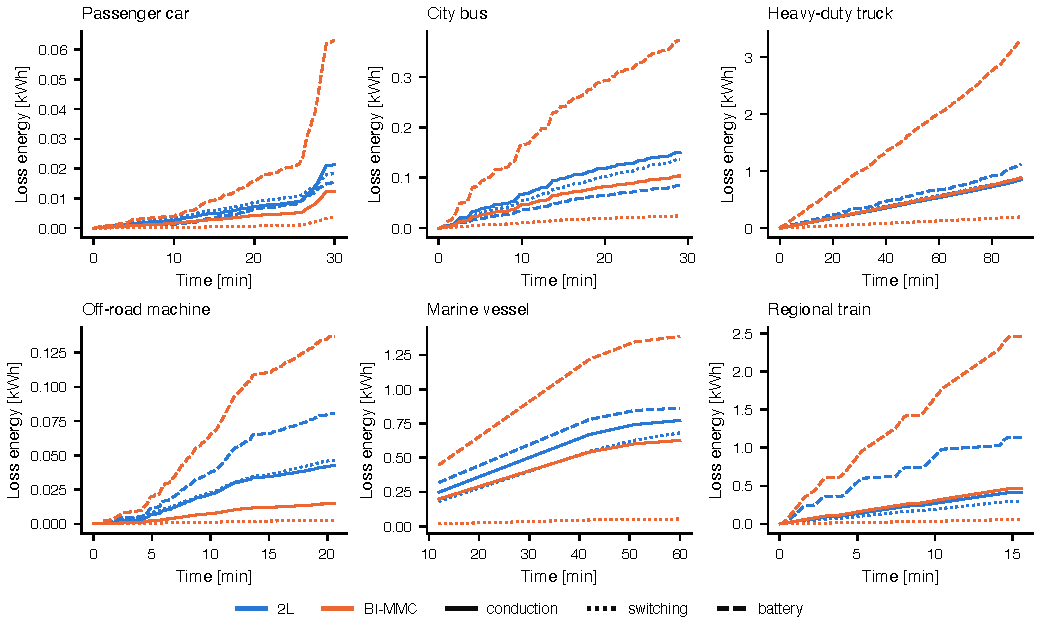
\includegraphics[width=\linewidth]{figures/paper_loss_energy.pdf}
\caption{Cumulative loss energy along each cycle (\SI{50}{\percent} initial SOC): conduction (solid), switching (dotted) and battery (dashed) loss of the 2L inverter (blue) and the BI-MMC (orange).}
\label{fig:lossenergy}
\end{figure}

\subsection*{Time series}
\begin{figure}[H]
\centering
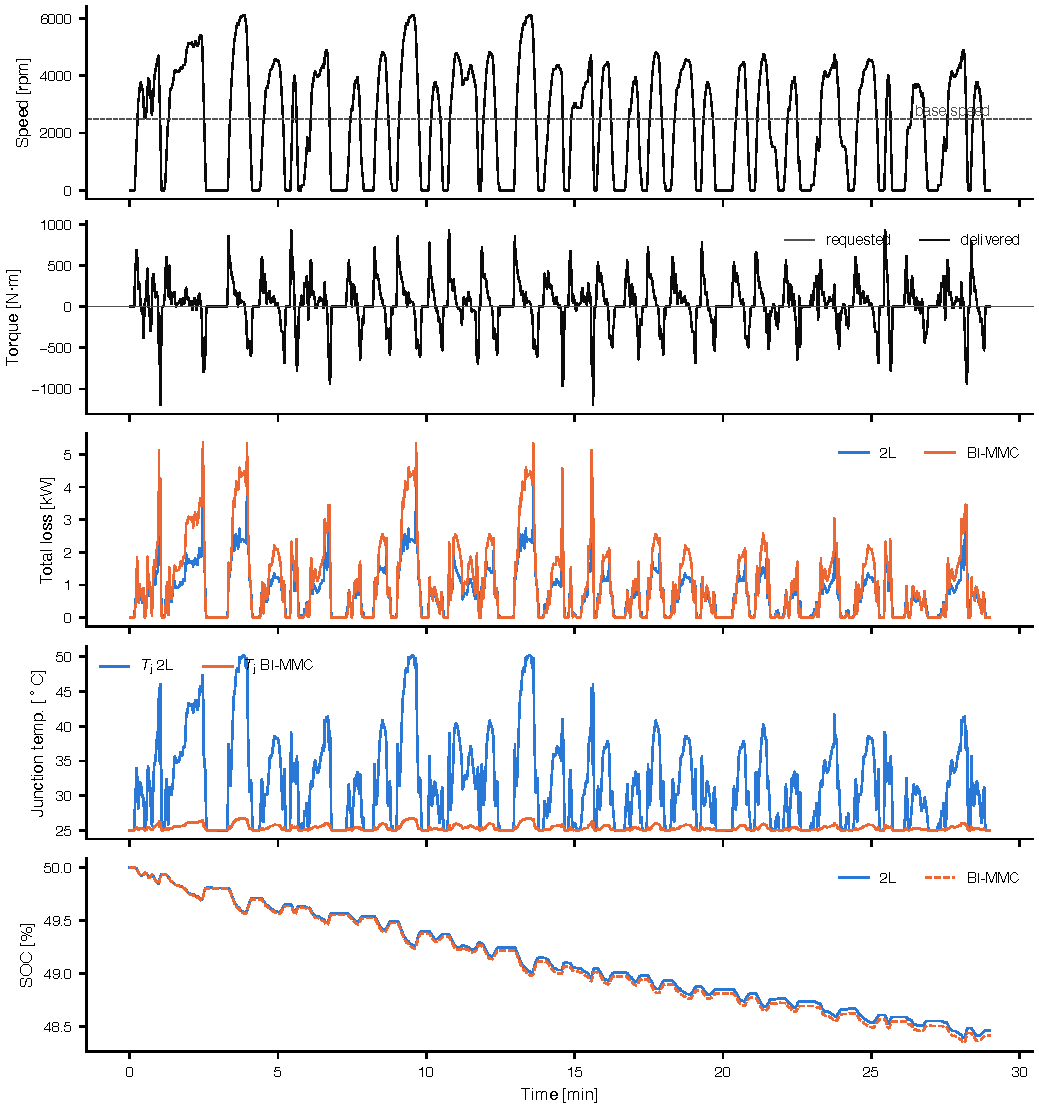
\includegraphics[width=0.88\linewidth]{figures/paper_trace_bus.pdf}
\caption{Time series of the city bus (Braunschweig, \SI{50}{\percent} initial SOC). The speed spikes above base speed are short, but the regenerative torque peaks are large.}
\end{figure}
\begin{figure}[H]
\centering
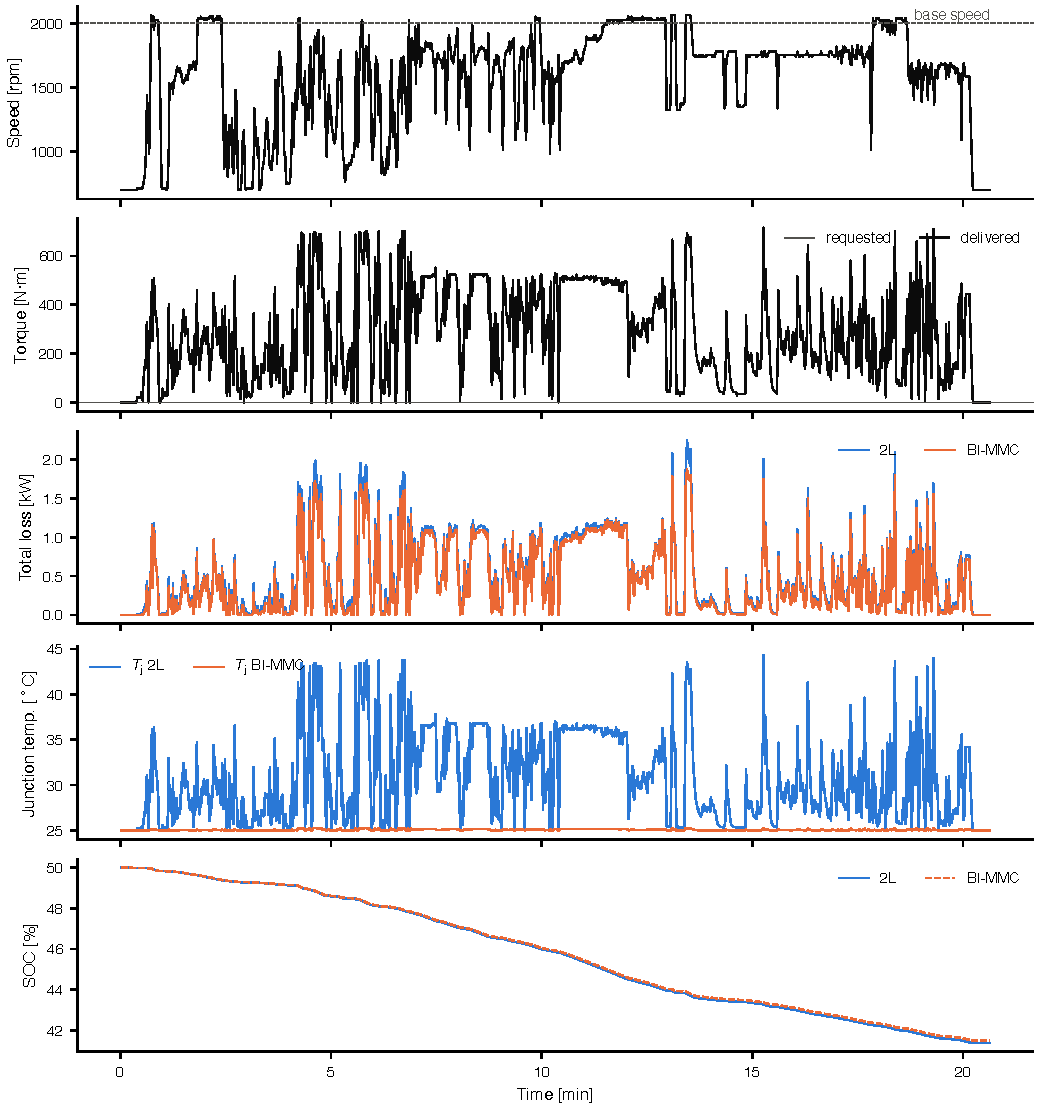
\includegraphics[width=0.88\linewidth]{figures/paper_trace_offroad.pdf}
\caption{Time series of the off-road machine (NRTC, \SI{50}{\percent} initial SOC).}
\end{figure}
\begin{figure}[H]
\centering
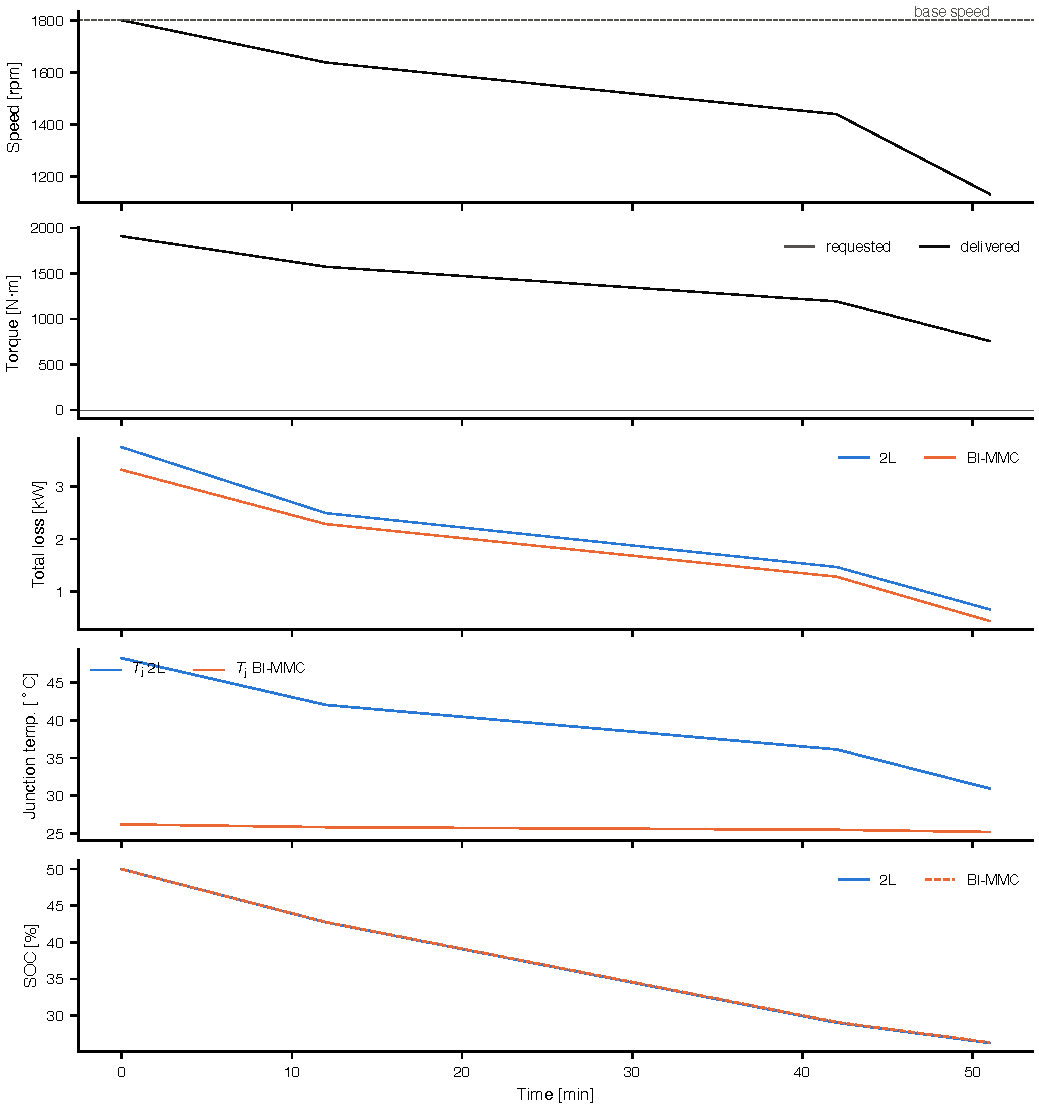
\includegraphics[width=0.88\linewidth]{figures/paper_trace_marine.pdf}
\caption{Time series of the marine vessel (ISO 8178 E3 modes, \SI{50}{\percent} initial SOC): four steady modes.}
\end{figure}
\begin{figure}[H]
\centering
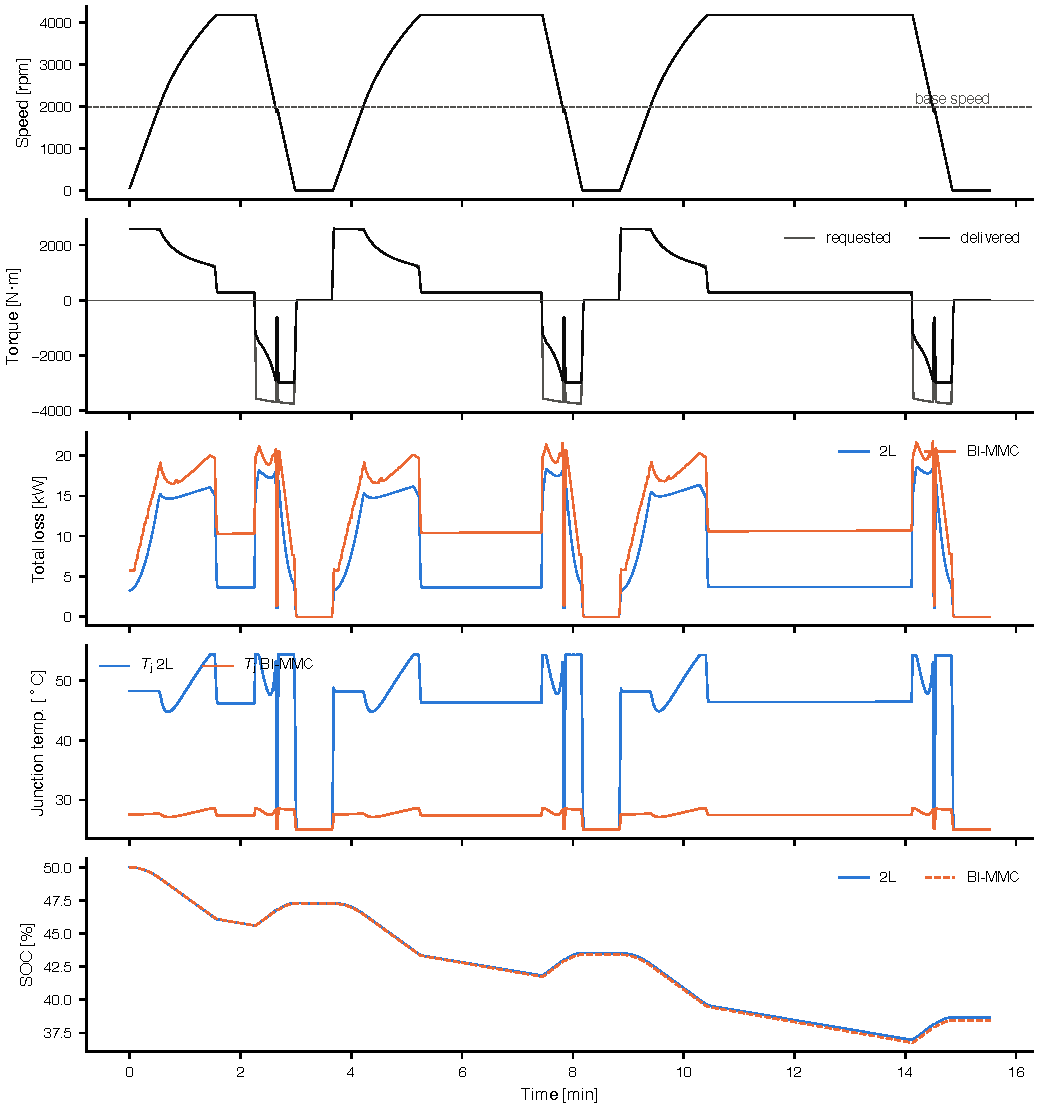
\includegraphics[width=0.88\linewidth]{figures/paper_trace_train.pdf}
\caption{Time series of the regional train (synthetic run, \SI{50}{\percent} initial SOC). The requested regenerative torque exceeds the torque limit, so the delivered torque is lower.}
\end{figure}

\subsection*{Efficiency maps of the remaining applications}
\begin{figure}[H]
\centering
\includegraphics[width=0.49\linewidth]{figures/maps/bus/efficiency_maps_comparison_soc_50.png}\hfill
\includegraphics[width=0.49\linewidth]{figures/maps/marine/efficiency_maps_comparison_soc_50.png}
\caption{Efficiency of the 2L inverter, the BI-MMC and their difference at \SI{50}{\percent} SOC for the city bus (left) and the marine vessel (right).}
\end{figure}
\begin{figure}[H]
\centering
\includegraphics[width=0.49\linewidth]{figures/maps/train/efficiency_maps_comparison_soc_50.png}\hfill
\includegraphics[width=0.49\linewidth]{figures/maps/train/losses_maps_comparison_soc_50.png}
\caption{Regional train at \SI{50}{\percent} SOC: efficiency of both drives and their difference (left), and total losses of both drives and their difference (right).}
\end{figure}
